%% bare_jrnl.tex
%% V1.4b
%% 2015/08/26
%% by Michael Shell
%% see http://www.michaelshell.org/
%% for current contact information.
%%
%% This is a skeleton file demonstrating the use of IEEEtran.cls
%% (requires IEEEtran.cls version 1.8b or later) with an IEEE
%% journal paper.
%%
%% Support sites:
%% http://www.michaelshell.org/tex/ieeetran/
%% http://www.ctan.org/pkg/ieeetran
%% and
%% http://www.ieee.org/

%%*************************************************************************
%% Legal Notice:
%% This code is offered as-is without any warranty either expressed or
%% implied; without even the implied warranty of MERCHANTABILITY or
%% FITNESS FOR A PARTICULAR PURPOSE! 
%% User assumes all risk.
%% In no event shall the IEEE or any contributor to this code be liable for
%% any damages or losses, including, but not limited to, incidental,
%% consequential, or any other damages, resulting from the use or misuse
%% of any information contained here.
%%
%% All comments are the opinions of their respective authors and are not
%% necessarily endorsed by the IEEE.
%%
%% This work is distributed under the LaTeX Project Public License (LPPL)
%% ( http://www.latex-project.org/ ) version 1.3, and may be freely used,
%% distributed and modified. A copy of the LPPL, version 1.3, is included
%% in the base LaTeX documentation of all distributions of LaTeX released
%% 2003/12/01 or later.
%% Retain all contribution notices and credits.
%% ** Modified files should be clearly indicated as such, including  **
%% ** renaming them and changing author support contact information. **
%%*************************************************************************


% *** Authors should verify (and, if needed, correct) their LaTeX system  ***
% *** with the testflow diagnostic prior to trusting their LaTeX platform ***
% *** with production work. The IEEE's font choices and paper sizes can   ***
% *** trigger bugs that do not appear when using other class files.       ***                          ***
% The testflow support page is at:
% http://www.michaelshell.org/tex/testflow/



\documentclass[journal]{IEEEtran}
\usepackage[brazilian]{babel}
\usepackage[utf8]{inputenc}
\usepackage[T1]{fontenc}
\usepackage{algorithm}
\usepackage{algpseudocode}
\usepackage{listings}
\usepackage{float}
\usepackage{color}

\floatname{algorithm}{Código}
\algrenewcommand\algorithmicfunction{\textbf{function}}
\algrenewtext{EndFunction}{\algorithmicend}
\algrenewtext{EndIf}{\algorithmicend}


\definecolor{mygreen}{rgb}{0,0.6,0}
\definecolor{mygray}{rgb}{0.5,0.5,0.5}
\definecolor{mymauve}{rgb}{0.58,0,0.82}

\lstset{ %
  backgroundcolor=\color{white},   % choose the background color; you must add \usepackage{color} or \usepackage{xcolor}; should come as last argument
  basicstyle=\footnotesize,        % the size of the fonts that are used for the code
  breakatwhitespace=false,         % sets if automatic breaks should only happen at whitespace
  breaklines=true,                 % sets automatic line breaking
  % captionpos=a,                    % sets the caption-position to bottom
  % commentstyle=\color{mygreen},    % comment style
  deletekeywords={...},            % if you want to delete keywords from the given language
  escapeinside={\%*}{*)},          % if you want to add LaTeX within your code
  extendedchars=true,              % lets you use non-ASCII characters; for 8-bits encodings only, does not work with UTF-8
  % frame=single,	                   % adds a frame around the code
  keepspaces=true,                 % keeps spaces in text, useful for keeping indentation of code (possibly needs columns=flexible)
  % keywordstyle=\color{blue},       % keyword style
  language=Octave,                 % the language of the code
  morekeywords={*,...},            % if you want to add more keywords to the set
  numbers=left,                    % where to put the line-numbers; possible values are (none, left, right)
  numbersep=-5pt,                   % how far the line-numbers are from the code
  numberstyle=\tiny\color{mygray}, % the style that is used for the line-numbers
  rulecolor=\color{black},         % if not set, the frame-color may be changed on line-breaks within not-black text (e.g. comments (green here))
  showspaces=false,                % show spaces everywhere adding particular underscores; it overrides 'showstringspaces'
  showstringspaces=false,          % underline spaces within strings only
  showtabs=false,                  % show tabs within strings adding particular underscores
  % stepnumber=2,                    % the step between two line-numbers. If it's 1, each line will be numbered
  % stringstyle=\color{mymauve},     % string literal style
  % tabsize=2,	                   % sets default tabsize to 2 spaces
  title=\lstname                   % show the filename of files included with \lstinputlisting; also try caption instead of title
}

\ifCLASSINFOpdf
  \usepackage[pdftex]{graphicx}
  % declare the path(s) where your graphic files are
  \graphicspath{{./img/}}
  % and their extensions so you won't have to specify these with
  % every instance of \includegraphics
  \DeclareGraphicsExtensions{.pdf,.jpg,.jpeg,.png}
\else

\fi

\hyphenation{op-tical net-works semi-conduc-tor}


\begin{document}

\title{IoT - A Internet das coisas}


\author{Willian Marques Freire e
        Munif Gebara Junior% <-this % stops a space
\thanks{Faculdade de Filosofia Ciências e Letras de Mandaguari é uma fundação
situada em Mandaguari no Paraná região sul brasileira,
na rua Rene Taccola, 152 - Centro Site: (see http://www.fafiman.br/index.html).}% <-this % stops a space
\thanks{Artigo realizado em 2017.}}



% The paper headers
\markboth{IoT - A Internet das Coisas,~Vol.~1, No.~1, Julho~2017}%
{Shell \MakeLowercase{\textit{et al.}}: Bare Demo of IEEEtran.cls for IEEE Journals}

\maketitle

% As a general rule, do not put math, special symbols or citations
% in the abstract or keywords.
\begin{abstract}
Este artigo têm por objetivo apresentar de maneira prática o desenvolvimento de uma estrutura IoT \emph{(Internet Of Things)}, que tenha por finalidade a fácil configuração de dispositivos integrados. Um dos maiores problemas quando se trata de IoT, são as configurações iniciais complexas que são necessárias de ser feitas. Sendo assim, surgiu a necessidade de utilizar tecnologias atuais que possibilitam o desenvolvimento do mesmo, de maneira prática e simples. Foram realizados diversos teste, e pesquisa de dispositivos IoT que atendam os requisitos mínimos de recursos para desenvolvimento da arquitetura, e optou-se a utilização do dispositivo integrados NodeMCU ESP8266 pois contém módulo Wi-Fi, além dos recursos necessários. Todo este assunto, e a arquitetura será tratado durante este artigo, e ao fim do mesmo será apresentado os resultados da pesquisa e desenvolvimento.
\end{abstract}

% Note that keywords are not normally used for peerreview papers.
\begin{IEEEkeywords}
IoT, Internet, Coisas.
\end{IEEEkeywords}




\IEEEpeerreviewmaketitle



\section{Introdução}

\IEEEPARstart{A} Internet têm transcorrido por diversas etapas evolucionárias distintas. A primeira fase existente foi quando a Web foi chamada de ARPANET \emph{(Advanced Research Projects Agency Network)}. A segunda fase da Web foi caracterizada pela concentração de todas as empresas, para compartilharem informações na Internet com intuito de divulgação de produtos e serviços. Seguido por uma terceira evolução, que mudou a Web, de um estágio com informações estáticas, para informações transacionais, nas quais produtos e serviços são comercializados totalmente online. Após todas estas evoluções, surge a quarta etapa, onde é criado o conceito de Web social e experiência do usuário, na qual empresas como Facebook e Twitter se tornaram famosas e profícuas, ao permitir que pessoas se comuniquem e compartilhem informações \cite[p.~6]{Evans}.

Considerando estas evoluções tecnológicas, IoT ou Internet das coisas, algumas vezes referida como a Internet dos objetos, também têm revolucionado, mudando o modelo de \emph{hardware} computacional, que nasceu a aproximadamente 40 anos atrás. Dentre todas as fases diferentes de modelos de \emph{hardware} que existiram, comprova-se que a cada revolução IoT, surge a necessidade de modificar este modelo \cite[p.~6]{dzonevoltreeiot}. Devido a diversos estudos visando o melhor desenvolvimento e aproveitamento do modelo cliente-servidor, surgiram vários protocolos para transmissão de dados, e o protocolo principal utilizado atualmente é o HTTP \emph{(Hypertext Transfer Protocol)}, encontrando-se por padrão em praticamente quase todos os navegadores atuais. Existem ainda outros protocolos como FTP \emph{(File Transfer Protocol)} para transferência de arquivos, IMAP \emph{(Internet Message Access Protocol)} para envio de Mensagens, entre outros. 

Aproveitando-se destes protocolos, também surgiram especificações e arquiteturas, para que aplicações possam ser disponibilizadas como serviços. Dentre elas encontra-se o REST \emph{(Representational State Transfer)} ou Transferência de Estado representacional, que segundo Fielding \cite{roythomasfielding2017}, é uma abstração da arquitetura World Wide Web, um estilo  arquitetural, que consiste em um conjunto coordenado de restições aplicadas a componentes, conectores e elementos de dados dentro de um sistema de hipermídia distribuído, entretanto, é um assunto para um próximo trabalho.

Considerando que o IoT representa a próxima evolução da Internet, melhorando a capacidade de coletar, analisar e distribuir dados, faz-se com que os mesmos possam ser transformados em informação. Atualmente existem projetos IoT em desenvolvimento, que prometem fechar a lacuna entre ricos e pobres, melhorando a distribuição dos recursos mundiais para aqueles que precisam deles, e ajudando a entender a sociedade atual para que possa ser mais proativa e menos reativa \cite[p.~2]{Evans}. Em 2003, haviam aproximadamente 6.3 bilhões de pessoas vivendo no mundo, e aproximadamente 500 milhões de dispositivos conectados à internet. O crescimento de smartphones e tablets, elevou o número de dispositivos conectados a Internet para aproximadamente 12,5 bilhões em 2010 \cite[p.~3]{Evans}.

\begin{figure}[H]
\centering
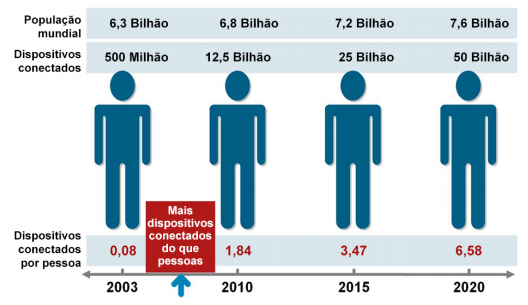
\includegraphics[width=2.5in]{um}
\caption{"Nascimento" do IoT entre 2008 e 2009 \cite{Evans}.}
\label{fig_um}
\end{figure}

Anteriormente, em janeiro de 2009, uma equipe de pesquisadores chinesa, finalizou um estudo sobre os dados de roteamento da internet em intervalos de seis meses, e foi descoberto pelos mesmos, que a Internet dobra de tamanho a cada 5,32 anos (EVERS, 2003). Na figura \ref{fig_um}, é possível observar o refinamento desta pesquisa. Devido a este crescimento no número de dispositivos conectados a internet, no artigo Internet of Things volume III, publicado pela empresa Dzone (empresa que faz publicações online sobre tecnologia) no ano de 2017, foi feito uma pesquisa interna na área de IoT. Na mesma, encontram-se 797 profissionais que são responsáveis por esta área, e foi questionado sobre as maiores preocupações quando se trata de IoT. O centro de preocupação estava pela segurança e privacidade, pois os mesmos, estavam interessados em IoT para o contexto empresarial de suas empresas. A falta de padrões, era um terço na coluna ''muito preocupada'' chegando a 34\% dos envolvidos. Dentre eles, 25\% dos entrevistados também  desconfiam da conectividade e do baixo custo de energia, sendo que 24\% se preocupam com a manutenção de \emph{hardware} e \emph{software}, e 14\% estão apreensivos com o desenvolvimento imaturo e paradigmas de redes \cite[p.~4]{Evans}.

O objetivo deste trabalho, é exemplificar o processo de criação de uma estrutura IoT, e demonstrar a resolução da lacuna de configuração de um dispositivo IoT de forma simples. Será desenvolvido durante este trabalho uma estrutura IoT flexível, que seja capaz de se comunicar através do protocolo HTTP com serviços WEB, que ficarão encarregados de compartilhar as informações recebidas dos dispositivos IoT pela Internet. Este artigo está organizado da seguinte forma: primeiramente será feito uma revisão bibliográfica sobre os assuntos que serão tratados, posteriormente será desenvolvido uma estrutura IoT que vise a fácil configuração da mesma, será feito também uma apresentação de resultados e por fim a conclusão deste artigo.

% \hfill 13 de Maio de 2017

\subsection{Revisão Bibliográfica}
\subsubsection{IoT}

Atualmente, existem diversos tipos e marcas de placas com circuito integrado e computadores, para desenvolvimento IoT. Em uma nova pesquisa realizada pelo Dzone, foram entrevistadors diversas pessoas, para obter um percentual de preferência entre dispositivos. Dentre os mesmos, 53\% preferem Rapberry Pi, 28\% preferem o Arduino, e 19\% não apresentam nenhuma preferência. Nesta pesquisa, foram relatados protocolos mais utilizados dentro do ramo IoT. Dentre os entrevistados, 14\% disseram ter preferência por Wifi-Direct em produção, 8\% preferem utilizar Bluetooh LE em ambientes que não são de produção. No total, 24\% já havia utilizado Wifi-Direct e 23\% Bluetooth LE. Um protocolo também citado, é o MQTT \emph{(Message Queue Telemetry Transport)}, que segundo o site FilipeFlop \cite{filipeflopnodemcu}, é um protocolo de mensagens leve, criado para comunicação M2M \emph{(Machine to Machine)}, que obteve 33\% de preferência de utilização em produção \cite[p.~4]{dzoneiotvolume4}.

Assim como aplicações web ou móveis, dispositivos físicos também precisam ser consensuais. No entanto, existem desafios adicionais para o IoT. As arquiteturas atuais ainda deixam a desejar em questão de terminais e configuração. Uma segunda preocupação na área de IoT é o tempo necessário para atualização de software para o dispositivo. Dentre as complicações que poder existir, a vulnerabilidade de um dispositivo, pode ser alvo para ataques e invasões. Uma das maneiras de gerenciar a testabilidade do software no dispositivo, é testar isoladamente. Reproduzir o ecossistema em torno do dispositivo e como os usuários interagem garantem uma boa testabilidade. Estudos avançados reconhecem que não se podem identificar, e muito menos testar cada possível cenário de falha. Por este fato, estes estudos concentram cada vez mais na confiabilidade e segurança IoT. O ultimo desafio para esta área, são as identificações e dignosticação de falhas. Tomar ações rapidamente para resolução de problemas, é um aspecto fundamental no desenvolvimento de dispositivos IoT. Técnicas para integração continua são utilizados para resolver estes problemas, e uma delas é a \emph{Canary Release}, que Segundo Danilo Sato \cite{danilosato2017}, é uma técnica para reduzir o risco de introduzir uma nova versão de software na produção, lançando mudanças lentamente para um pequeno subconjunto de usuários, antes de lança-la em toda a infra-estrutura e torná-la disponível para todos \cite[p.~9]{dzoneiotvolume4}.

Nas últimas duas décadas, houveram avanços tecnológicos na área computacional, surgindo processadores com mais capacidade, armazenamentos, memória e dispositivos de rede com baixo custo. Atualmente, dispositivos físicos estão sendo desenvolvidos com mais capacidade computacional, e interligados através da internet de maneira efetiva. A adoção generalizada das tecnologias IoT enriquecem a idéia de computação ubíqua, um conceito que surgiu no final dos anos 80. Mark Weiser, criador deste conceito, escreveu em seu artigo The Computer for the 21st Century, que o computador se integra a vida das pessoas de modo que elas não o percebam, todavia, o utilizam. Motivado por esta convicção, Weiser percebeu que em sua época não haviam tecnologias necessárias para que a Computação Ubíqua se tornasse realidade, fazendo com que assim, dedicasse esforços para desenvolver estes meios. \cite{MarkWeiser}.

Após alguns anos, no início de 1926, uma revista chamada Collier publicou uma entrevista com Nikola Tesla, no qual ele falou sobre suas previsões para as próximas décadas. Entre elas, ele falava de um mundo com máquinas voadoras, energia sem fio e superioridade feminina. Segundo palavras de Tesla,s quando a tecnologia sem fio estivesse perfeitamente estabelecida em todo o mundo, o planeta se tornaria um enorme cérebro. Nesta entrevista, ele disse que inclusive os seres humanos seriam capazes de se comunicar uns com os outros de imediato, independente da distância \cite{johnBKennedy}.

Além disto, em um artigo feito pelo professor Michael Wooldridge (chefe do Departamento de Ciência da Computação da Universidade de Oxford), definiu um termo utilizado no meio tecnológico, que são os agentes. Segundo ele, um agente é um computador que está situado em algum ambiente, capaz de realizar ações autônomas sobre este, para cumprir seus objetivos delegados. O mesmo torna-se inteligente com as seguintes propriedades: Reatividade (a percepção de seu ambiente, e a capacidade de respota em tempo hábil sobre mudanças que ocorrem), proatividade (antecipação de problemas futuros), habilidade social (capacidade de interação entre agentes para satisfazer seus objetivos de design) \cite{MichaelWooldridge}.

\subsubsection{NodeMCU}

Neste trabalho, será utilizado o NodeMCU para desenvolvimento das aplicaçoes IoT, pelo fato do mesmo conter um módulo WiFi, o que facilitará na comunicação via interface de rede com outros dispositivos. NodeMCU é um firmware baseado em eLua (implementação completa utilizando programação Lua para sistemas embarcados) \cite{elua2017}. O mesmo foi projetado para ser integrado com o Chip WiFi ESP8266 desenvolvido pela empresa Espressif, situada em Shangai, especializada no ramo de IoT \cite{systems}. O NodeMCU utiliza sistema de arquivos SPIFFS \emph{(SPI Flash File System)} e seu repositório no Github consiste em 98.1\% de código na linguagem C - criada em 1972 por Dennis Ritchie \cite{williamstewart2017} e o demais existente em código escrito na linguagem Lua  - criada em 1993 por Roberto Ierusalimschy, Luiz Henrique de Figueiredo e Waldemar Celes \cite{lua2017Authors}.

ESP8266 é um chip com arquitetura 32 bits, e o seu tamanho está em 5mm x 5mm. Existem diversos módulos parecidos. Dentre eles estão, o ESP-01 que contém 8 conectores, e surgiu para ser utilizado como um módulo para o Arduino, o ESP-07 que contém 16 pinos, antena, cerâmica e conector para antena externa, e o ESP-12E, que conta com 22 pinos, que possibilita a ligação de diversos módulos ao ESP como \emph{displays}, cartões SD, dentre outros. Um ponto importante nestes módulos, é que eles utilizam 3,3V. Comparado ao Arduino UNO, o NodeMCU se destaca por ter um processador Tensilica LX106, que pode atingir até 160MHZ, e possui uma memória RAM de 20KB e uma memória flash de 4MB. Já o Arduino UNO possui um micro controlador de 16MHZ, possui uma memória RAM de 2KB e uma memória flash de 32KB. Outra questão a ser levado em conta, é o custo benefício, pois atualmente é possível encontrar o ESP8266 por até US\$1,70, e um Arduino UNO ultrapassa os 20 dólares\cite{IrvingNodeMCU}.


\subsubsection{Módulo Wi-Fi}

Devido ao elevado número de cabos necessários para interconectar computadores e dispositivos, surgiu o WiFi. É muito utilizado cabos, entretanto possuem algumas limitações. Um exemplo é o deslocamento dos mesmos, é trabalhoso pelo fato de possuir limite de alcance, e em ambientes com muitos computadores, são necessárias apropriações estruturais. O uso do Wi-Fi tem se tornando comuns nao somente em residências, mas também em ambientes corporativos e públicos. Dentre os padrões de Wi-Fi existentes, estão o 802.11b que tem como possibilidade p estabelecimento de conexões nas seguintes velocidades de transmissão: 1 Mb/s, 2Mb/s, 5,5 Mb/s e 11 Mb/s, o 802.11g que surgiu em 203 e é totalmente compatível com o 802.11b, e possui como atrativo a possibilidade de trabalhar com taxas de transmiss~ao de até 54 Mb/s, o 802.11n que tem como principal característica a utilização de um esquema chamado MIMO ou \emph{Multiple-Input Multiple-Output}, que é capaz de atingir taxas de transmissão de até 600 Mb/s, e finalmente o 802.11ac, também chamado 5G WiFi, que sua principal vantagem está em sua velocidade, estimada em até 433 Mb/s no modo mais simples, fazendo com que, é possível fazer a rede suportar 6 Gb/s  de velocidade na trasmiss~ao de dados. Resumidamente, Wi-Fi é um conjunto de especificaçoes para redes locais sem fio baseada no padrão IEEE 802.11, uma abreviatura para \emph{''Wireless Fidelity''}. \cite{wifiinfowester}

\subsubsection{Segurança Wi-Fi}

Apesar de todas as facilidades que se encontram ao utilizam tecnologias sem fio como Wi-Fi, assim como todo sistemas, medidas de segurança devem ser utilizadas para previnir ataques e invasões. Existem protocolos de segurança que auxiliam na segurança de conexões Wi-Fi, dentre eles se encontram: WEP, WPA, e o WPA2. \emph{Wired Equivalent Privacy} (WEP) é um algoritmo de segurança que foi criado em 1999 e é compatível com prativamente todos os dispositivos Wi-Fi disponível no mercado. Este padrão se torna mais inseguro à medida que o poder de processamento dos computadores aumenta. Pelo fato de conter um numero máximo de combinações de senha totalizando 128 bits, é possível descobrir a palavra-passe em poucos minutos por meio de softwares de ataques. \emph{Wi-Fi Protected Access} ou WPA, surgiu quando o WEP saiu de circulação, e entrou como protocolo-padrão industrial. Adotado em 2003, trazia como novidade a encriptação 256 bits e como segurança adicional, fazia análise de pacotes, para verificar alterações e invasões. Atualmente é utilizado o \emph{Wi-Fi Protected Access II} ou WPA2, pelo fato de ser o mais seguro. Foi implementado pela Wi-Fi Alliance em 2006, e possui como diferencial a maneira como lida com senhas e algoritmos, excluindo totalmente a possibilidade de um ataque de força bruta. Segundo especialistras, o riscos de intrusos em redes domésticos é quase zero. Isto se deve a utilizição de duas tecnologias que são utilizadas neste algoritmo, o AES (Advanced Encryption Standard) que é um novo padrão para segurança das informações, e o CCMP \emph{(Counter Cipher Mode)}, um mecanismo de encriptação que protege os dados que passam pela rede. Devido a complexidade do mesmo, muitos dispositivos, mesmos recentes, não são compatíveis com ele. \cite{wifitecmundo}

\subsubsection{Sistema de arquivos}

O NodeMCU utiliza o sistema de arquivos SPIFFS, um sistema de arquivos destinado a dispositivos \emph{flash} embarcados. SPIFFS é projetado para projetos que são pequenos e memória sem pilha \cite{SPIFFS}. O projeto pode ser clonado do repositório do mesmo no github.

\subsubsection{Ferramenta para desenvolvimento}

Neste projeto será utilizado uma ferramenta chamada ESPlorer. ELa é utlizada para facilitar o desenvolvimento de aplicações LUA para dispostivos ESP8266. Basicamente, é uma IDE (Ambiente de desenvolvimento integrado), que possui diversos facilitadores para melhor visualização do código e envio do código fonte para o dispositivo. Esta ferramenta possui um terminal para \emph{debug}, e acessos rápidos para executar comandos. Nela também é possível executar comandos de forma rápida. Todos estes fatores beneficiaram na escolha de utilização desta ferramenta para o desenvolvimento do trabalho \cite{ESPlorer}. Na figura \ref{esplorer} é possível observar estas características.

\begin{figure}[h]
\centering
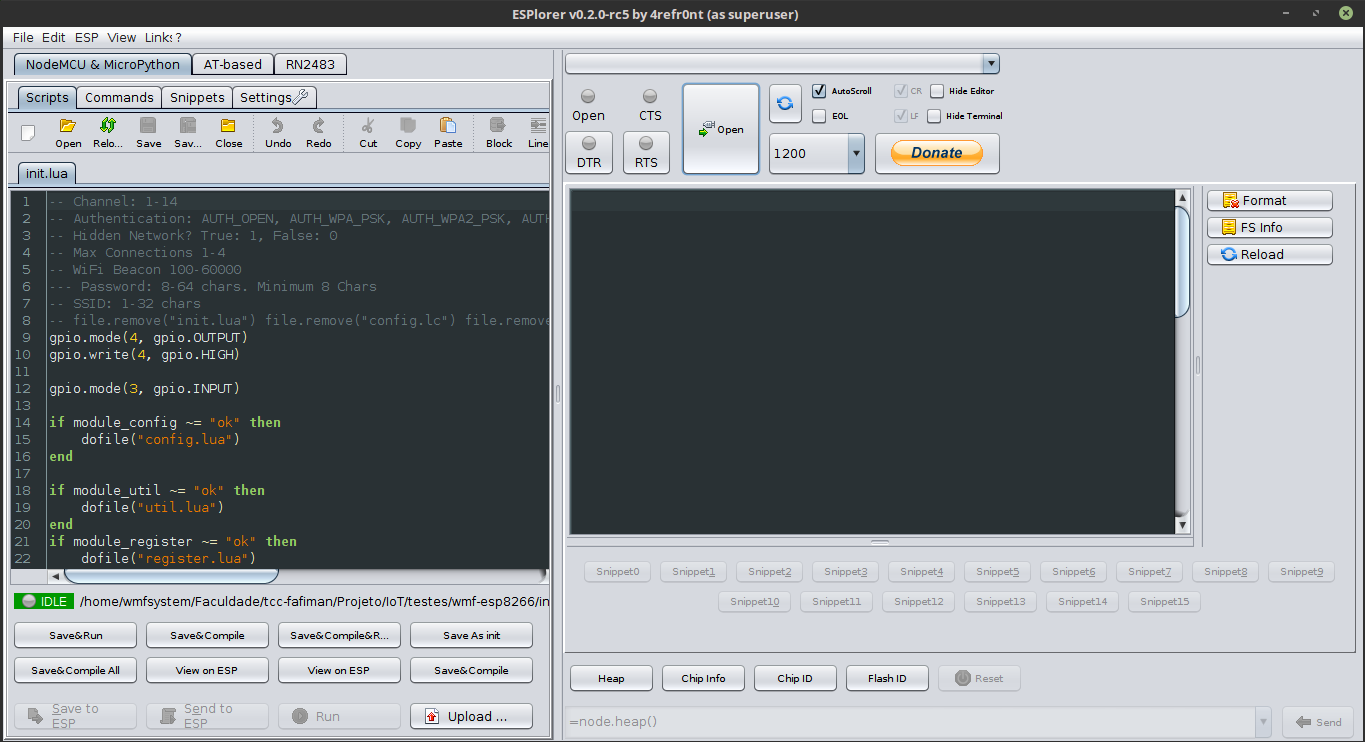
\includegraphics[width=2.5in]{esplorer}
\caption{Esplorer \cite{ESPlorer}}
\label{esplorer}
\end{figure}

\subsubsection{Protocolos TCP e UDP}
O protocolo TCP ou Protocolo de controle de transmissão, é um dos protolocos mais utilizados. Ele é complementado pelo IP (Protocolo da Internet), sendo normalmente chamado de TCP/IP. A versatilidade e robustez do mesmo tornou-o mais adequado para utilização em redes globais, já que são feito verificação de dados para confirmação de recebimento e entrega sem erros. O TCP é um protocolo que se encontra no nível da camada 4 ou camada de transporte do modelo OSI (sistema de interconexão aberto), que é um modelo de referência da ISO (Organização Internacional para Padronização) dividido em camadas de funções, que são: Aplicação que fornece serviços às aplicações do cliente, Apresentação que fornece encriptação e compressão de dados, além de garantir a compatibilidade entre camadas de aplicação de sistemas diferentes, Sessão que controla as sessões entre aplicações, transporte que controla o fluxo de informação e controle de erros, rede que encaminha pacotes e possui esquema de endereçamentos, dados que controla o acesso o meio físico de tansmissão e erros da camada física, e finalmente a camada física, que define as características do meio físico de transmissão da rede, conectores, interfaces, codificação ou modulação de sinais \cite{pplwareosi}\cite{VintonTCP}.

Outro protocolo que também será utilizado, é o UDP \emph{(User Datagram Prococol)}. Antes de entender a diferença do UDP para o TCP é necessário saber o que é um datagrama. Segundo a RFC 1594 \cite{rfc1594} é uma entidade de dados completa e independente que contém informações suficientes para ser roteada da origem ao destino sem precisar confiar em trocas anteriores entre essa fonte, a máquina de destino e a rede de transporte. O UDP permite que a aplicação envie um datagrama encapsulado em um Pacote IPv4 ( ou IPv6, e então enviado ao destino. Ao contrário de TCP, no UDP não há qualquer tipo de garantia que o pacote será entregue.

% needed in second column of first page if using \IEEEpubid
%\IEEEpubidadjcol


\subsection{Desenvolvimento}
\subsubsection{Configurações iniciais no NodeMCU ESP-8266}
Primeiramente, para se utilizar este dispositivo, é necessário fazer o build (compilação) do firmware, conforme a figura \ref{alg:modulesh}, pois o mesmo é distribuido sem nenhum sistema operacional. Atualmente, pode-se fazer o build do mesmo utilizando o site \emph{https://nodemcu-build.com} ou clonar o repositório do projeto do github. No caso deste projeto, o build do projeto será feito manualmente. Para incluir bibliotecas neste módulo, é necessário editar o arquivo que se encontra no diretório \emph{app/include/user\_modules.h} do projeto e retirar os comentários das bibliotecas que será utilizado.

\begin{figure}[h]
\centering

\begin{lstlisting}[language=C]
  #define LUA\_USE_MODULES\_MQTT
  // #define LUA\_USE\_MODULES_COAP
  // #define LUA\_USE\_MODULES\_U8G
\end{lstlisting}

\caption{Compilação do firmware}
\label{alg:modulesh}
\end{figure}

Duas possibilidades disponível pelo módulo NodeMCU, são ativar o suporte TLS e o debug (depurador) quando em execução. Para utilizar o suporte TLS, é necessário descomentar a opção \emph{CLIENT\_SSL\_ENABLE} que se encontra dentro do arquivo \emph{user\_config.h} no diretório app/include, e para ativar o modo debug em tempo de execução, e descomentar a linha em que se encontra \emph{\#define\ DEVELOP\_VERSION}.

Por padrão, o build do firmware é gerado com suporte a variáveis com ponto flutuante, entretanto, isto ocupa mais memória, e para reduzir a quantidade de memória utilizada, deve-se comentar em que é definido a constante \emph{LUA\_NUMBER\_INTEGRAL} dentro so arquivo \emph{user\_config.h}.

\subsubsection{Gerando e gravando o firmware}

Após ajustar as devidas configurações inicial, é necessário compilar e gravar o \emph{firmware} no dispositivo, conforme a figura \ref{alg:dockerpull}. Neste trabalho, será utilizado a ferramenta esptool para gravar o mesmo. Esta ferramenta pode ser encontrada no repositório da Espressif (empresa que desenvolveu o NodeMCU) no github, e foi iniciada por Fredrik Ahlbeg, um dos envolvidos no projeto, e atualmente é mantido por Angus Gratton e pela comunidade. E para compilar os códigos fontes, deve-se primeiramente executar os seguintes comandos dentro do diretório do projeto.

\begin{figure}[h]
\centering

\begin{lstlisting}[language=bash]
  $ docker pull marcelstoer/nodemcu-build
  $ sudo docker run --rm -ti -v `pwd`:/opt
  /nodemcu-firmware 
  marcelstoer/nodemcu-build
\end{lstlisting}

\caption{Compilação do firmware}
\label{alg:dockerpull}
\end{figure}


Como este projeto utiliza o docker, uma infraestrutura independente de plataforma \cite{dockeroque}, primeiramente é atualizado o container e posteriormente é executado um comando para compilar o projeto. 
Após compilado, deve ser executado os comandos conforme a figura \ref{alg:esptool1}, utilizando a ferramenta esptool. Estes comandos serão utilizados para gravar o firmware no ESP8266. 


\begin{figure}[H]
\centering

\begin{lstlisting}[language=bash]
  $ sudo python esptool.py 
      --port="/dev/ttyUSB1" 
      erase_flash

  $ sudo python ./esptool.py 
      --port /dev/ttyUSB0 
      write_flash 
      0x00000 
      ../nodemcu-firmware/bin/0x00000.bin 
      0x10000 
      ../nodemcu-firmware/bin/0x10000.bin

  $ sudo python ./esptool.py 
      --port="/dev/ttyUSB0" 
      write_flash -fm=dio 
      -fs=16m 0x00000 
      ./../nodemcu-firmware/bin
      /nodemcu_integer__20170510-0106.bin
\end{lstlisting}

\caption{Compilação do firmware}
\label{alg:esptool1}
\end{figure}


Os comandos da figura \ref{alg:esptool1} estão divididos em 3 partes. Primeiramente é removido todo o firmware do dispositivo, posteriormente é gravado nos endereçamentos 0x00000 e 0x10000 os arquivos com bibliotecas padrões utilizadas no firmware. Após isto é gravado o firmware com as bibliotecas extras selecionadas para inclusão no dispositivo.

\subsubsection{Access Point para configuração}

Assim como todo dispositivo, neste trabalho será desenvolvido uma central de configuração. Como este dispositivo foi desenvolvido com foco na utilização e conexão Wi-fi, será criado uma central para configuração sobre qual dispositivo Wireless o mesmo se conectará, e para isto, como a maioria destes dispositivos possuem regras de segurança e senhas, deverá conter também a opção para que seja configurado a senha do dispositivo. 

Um dos recursos que o ESP8266 provê, é o desenvolvimento de um AP (\emph{Access Point} ou ponto de acesso), que permite interligar duas ou mais redes sem fio. Dentre as diversas funções de um AP estão: repetir um sinal e transformar um sinal de um cabo em sinal sem fio \cite{accesspoint}. Entretanto, neste trabalho será utilizado somente como central para configuração do dispositivo.

Primeiramente é necessario fazer o NodeMCU trabalhar com o padrão Access Point. Ele provê um facilitador para que o dispositivo trabalhe como Access Point e como cliente. Para isto é necessário fazer conforme a figura \ref{alg:STATIONAP}. Neste trabalho será criado inicialmente um arquivo chamado \emph{init.lua}, onde se encontrará o código fonte que será executado ao iniciar o dispositivo.

\begin{figure}[h]
\centering

\begin{lstlisting}
  wifi.setmode(wifi.STATIONAP)
\end{lstlisting}

\caption{Configurando modo Access Point.}
\label{alg:STATIONAP}
\end{figure}

Uma outra possibilidade ao utilizar o NodeMCU, é a criação de um pequeno servidor em uma de suas portas. Neste caso, será criado um servidor TCP conforme a figura \ref{alg:TCPSERVER}, para que quando alguém se conectar no dispositivo em uma determinada porta padrão, esteja disponível a central de configuração caso o dispositivo não esteja conectado em nenhum roteador Wireless.

\begin{figure}[h]
\centering

\begin{lstlisting}
  srv = net.createServer(net.TCP)
\end{lstlisting}

\caption{Criando Servidor TCP.}
\label{alg:TCPSERVER}
\end{figure}

Uma das questões encontradas neste trabalho, foi a forma de como manter estas configurações em funcionamento, pois se ocorrer algo que faça com que o dispositivo desligue, seria interessante que o mesmo mantivesse as configurações salvas, para que não seja necessário a reconfiguração do Wi-Fi. Para isto, será utilizado o sistema de arquivos do ESP8266, para criação de um arquivo config.lc, conforme a figura \ref{alg:trimcc}, e sempre que o dispositivo iniciar, será feito a verificação da existência do arquivo de configurações para conexão do Wi-FI, e se caso não existir este arquivo, será iniciado a central de configuração do dispositivo.

Para configurar um Access Point, é necessário algumas considerações como: ssid (Nome da conexão), pwd (Senha da conexao), auth (Tipo de autenticação), channel (Canal que será liberado no dispositivo Wi-Fi), hidden (indica se é visível), max (máximo de conexões simutâneas) e beacon (intervalo de tentativas de conexão do dispositivo). Quando é encontrado o arquivo, é feito uma leitura do mesmo, e neste trabalho, está sendo salvo no padrão usuário e senha separados por um espaço em branco. Os demais códigos desenvolvidos, podem ser encontrados no apêndice deste trabalho. No arquivo \emph{init.lua} deverá ser feito a importação dos mesmos, pois serão divididos da seguinte forma: \emph{init.lua} (arquivo inicial), \emph{config.lua} (arquivo que terá o código de configuração) e util.lua (arquivo que terá funções utilitárias). Para importar os demais módulos, foi feito conforme a figura \ref{alg:importsdofile}.

\begin{figure}[H]
\begin{lstlisting} 
  dofile("config.lua")
  dofile("util.lua")
  dofile("register.lua")
\end{lstlisting}

\caption{Importação dos módulos}
\label{alg:importsdofile}
\end{figure}


\section{Resultados}
O NodeMCU ESP8266 possui um módulo Wi-Fi, o que possibilitou a conexão à rede de internet. O mesmo possui um sistema de arquivos, o que permitiu as configurações serem salvas no dispositivo, para que se caso ocorra alguma falha, ou até mesmo o dispositivo seja desligado, não seja necessário fazer novamente as configuraçãos iniciais. Foi implementado uma regra no dispositivo, que faz a verificação de conexão a internet dentro de 20 segundos, e se ocorrer algulma falha na conexão, será deletado o arquivo de configurações e reinicializado o dispositivo, liberando assim, o acesso à configuração de rede.

Como este dispositivo tem suporte a protocolos TCP e UDP, é aberto possibilidades para integração com outros dispositivos ou sistemas que utilizam este protocolo. Foram realizados diversos testes com o mesmo, dentre eles utilizando o GPIO \cite{nodemcugpio} para utilização de pinos digitais, SJSON para serialização de Objetos utilizandos textos no padrão JSON \cite{nodemcujson} e o Timer para executar funções em determinado tempo \cite{nodemcutimer}.

\section{Conclusões e trabalhos futuros}
Utilizando-se destes recursos disponíveis no NodeMCU ESP8266, é possível montar uma estrutura IoT flexível e de simples configuração. Atualmente existem outros dispositivos embarcados semelhantes que são acessíveis. Entretanto, neste trabalho foi utilizado este, pelo fato de ter um custo-benefício acessível, e de estar sendo utilizado pela comunidade. Foi utilizado a linguagem LUA para desenvolver neste dispositivo, entretanto, existem alguns projetos que possibilitam o desenvolvimento em outras linguagens. Como neste trabalho foi desenvolvido uma estrutura IoT de fácil configuração e com tecnologias como TCP e UDP, foi aberto possibilidades para o desenvolvimento de sistemas que se integrem com o mesmo, utilizando a rede de internet, e trabalhos futuros podem visar esta possibilidade. Sistemas complexos de automação residencial ou industrial podem ser resolvidos acoplando estas tecnologias, integrando o dispositivo com a rede de internet de forma fácil, foi resolvida.


\newpage
\appendices

\section{Código fonte Configuracional: config.lua}

\begin{figure}[H]
\centering

\begin{lstlisting}
  function configureWifi()
    local ap = {}
    wifi.sta.getap(
      function(t)
        i = 0
        for ssid, v in pairs(t) do
            ap[i] = ssid
            i = i + 1
        end
      end)
    srv:listen(
      80,
      function(conn)
        conn:on(
          "receive",
          function(conn, payload)
            listaAp = "SSID: <select name='ssid'>"
            print("Request Configuration")
            for i = 0, tablelength(ap), 1 do
              if ap[i] ~= nil then
                listaAp = listaAp 
                  .. "<option value='" 
                  .. ap[i] .. "'>" 
                  .. ap[i] .. "</option>"
              end
            end
            listaAp = listaAp .. "</select><br/>"
            
            local _GET = getParamsUrl(payload)
            
            if (_GET ~= nil) then
              if (_GET.ssid ~= nil 
                and _GET.password ~= nil) then
                print("Connecting to wifi 
                and creating configuration...")
                print("SSID: " 
                  .. _GET.ssid)
                print("Password: " 
                  .. _GET.password)
                
                for i = 0, tablelength(ap), 1 do
                  if ap[i] ~= nil then
                    if (string
                      .find(ap[i], _GET.ssid)) then
                      user = ap[i]
                    end
                  end
                end
                
                password = _GET.password
                wifi.sta.config(user, password)
                wifi.sta.connect()
                
                if file.open("config.lc", "w") then
                  file.writeline(user 
                    .. " " .. password)
                  file.close()
                end
                
                node.restart()
                node.chipid()
              end
            end
            conn:send([[... HTML Whatever...]]))
          conn:on("sent", function(conn)
            conn:close()
            collectgarbage()
          end)
      end)
  end
\end{lstlisting}

\caption{Módulo Utilitário}
\label{alg:configcondif}
\end{figure}

\section{Código fonte Utilitário: util.lua}


\begin{figure}[H]
\centering

\begin{lstlisting}
  function split(str, pat)
      local t = {} 
      -- NOTE: use {n = 0} in Lua-5.0
      local fpat = "(.-)" .. pat
      local last_end = 1
      local s, 
            e, 
            cap = str:find(fpat, 1)
      while s do
          if s ~= 1 or cap ~= "" then
              table.insert(t, cap)
          end
          last_end = e + 1
          s, 
          e, 
          cap = str:find(fpat, last_end)
      end
      if last_end <= #str then
          cap = str:sub(last_end)
          table.insert(t, cap)
      end
      return t
  end

  local unescape = function(s)
      s = string.gsub(s, "+", " ")
      s = string.gsub(
          s,
          "%%(%x%x)",
          function(h)
              return string.char(tonumber(h, 16))
          end
      )
      return s
  end

  function tablelength(T)
      local count = 0
      for _ in pairs(T) do
          count = count + 1
      end
      return count
  end

  function getParamsUrl(request)
      local buf = ""
      local 
        _, _, 
        method, 
        path, 
        vars = string
          .find(request, "([A-Z]+) (.+)?(.+) HTTP")
      if (method == nil) then
          _, _, 
          method, 
          path = string.find(request, "([A-Z]+) (.+) HTTP")
      end
      local _GET = {}
      if (vars ~= nil) then
          for k, v in string
            .gmatch(vars, "(%w+)=(%w+)&*") do
              _GET[k] = unescape(v)
          end
      end
      return _GET
  end
\end{lstlisting}

\caption{Módulo Configuracional}
\label{alg:configcondif}
\end{figure}

\section{Código fonte inicial: init.lua}

\begin{figure}[H]
\centering

\begin{lstlisting}

  srv = net.createServer(net.TCP)

  if file.exists("config.lc") == true then

      print("Open configuration...")

      if file.open("config.lc") then

          local corte = 
            split(file.read(), " ")
          user = corte[1]:gsub("%s+", "")
          password = corte[2]:gsub("%s+", "")
          
          print("Connecting in ip with user: " 
          .. user 
          .. " and password: " 
          .. password)
          wifi.sta.config(user, password)
          wifi.sta.connect()

      end

  else

      wifi.ap.config({
        ssid = "NodeMcuEsp8266"
          ..node.chipid(), 
        pwd = nil, 
        auth = AUTH_OPEN, 
        channel = 6, 
        hidden = 0, 
        max = 4, 
        beacon = 100
      })

      wifi.ap.setip({
        ip = "192.168.10.1", 
        netmask = "255.255.255.0", 
        gateway = "192.168.10.1"
      })

      wifi.ap.dhcp.config(
          {start = "192.168.10.2"}
      )

      tmr.alarm(
          1,
          1000,
          1,
          function()
              if wifi.ap.getip() == nil then
                  print("Connecting...")
              else
                  print("Connected in " 
                    .. wifi.ap.getip())
                  configureWifi()
              end
              tmr.stop(1)
          end
      )

  end



\end{lstlisting}

\caption{Central de Configuração}
\label{alg:trimcc}
\end{figure}


\ifCLASSOPTIONcaptionsoff
  \newpage
\fi


\begin{thebibliography}{1}

\bibitem{Evans}
Dave Evans. \emph The Internet of Things How the Next Evolution of the Internet Is Changing Everything, vol 1, pp. 2-4, 2011

\bibitem{MarquesMunif}
Willian Marques Freire e Munif Gebara Júnior. \emph Micro-serviços, vol 1, pp. 1-3, 2017

\bibitem{dzonevoltreeiot}
John Esposito. \emph The Dzone Guide to Internet of Things, vol 3, pp. 1-6, 2016

%Colocar neste padrão [Online]
\bibitem{wifiinfowester}
Emerson Alecrim. \emph O que é Wi-Fi (IEEE 802.11)? 2013 [Online] Disponível: https://www.infowester.com/wifi.php\#80211. [Acesso: 20-Mai-2017]

\bibitem{dockeroque}
Docker. \emph Docker 2017 [Online] Disponível: https://www.docker.com. [Acesso: 11-Jun-2017]

\bibitem{SPIFFS}
Peter Andersson. \emph SPIFFS (SPI Flash File System) 2013 [Online] Disponível: https://github.com/pellepl/spiffs. [Acesso: 11-Jun-2017]

\bibitem{ESPlorer}
ESPlorer. \emph ESPlorer Integrated Development Environment (IDE) for ESP8266 developers 2013 [Online] Disponível: https://github.com/4refr0nt/ESPlorer. [Acesso: 11-Jun-2017]

\bibitem{wifitecmundo}
Felipe Demartini. \emph WEP, WPA, WPA2: o que as siglas significam para o seu WiFi? 2013 [Online] Disponível: https://www.tecmundo.com.br/wi-fi/42024-wep-wpa-wpa2-o-que-as-siglas-significam-para-o-seu-wifi-.htm. [Acesso: 03-Jun-2017]

\bibitem{accesspoint}
Mundo Max. \emph Qual a diferença entre um Roteador Wireless e um Access Point? 2011 [Online] Disponível: http://www.mundomax.com.br/blog/informatica/qual-a-diferenca-entre-um-roteador-wireless-e-um-access-point/. [Acesso: 03-Jun-2017]

\bibitem{IrvingNodeMCU}
Irving Souza Lima. \emph NodeMCU (ESP8266) o módulo que desbanca o Arduino e facilitará a Internet das Coisas. 2016 [Online] Disponível
http://irving.com.br/esp8266/nodemcu-esp8266-o-modulo-que-desbanca-o-arduino-e-facilitara-a-internet-das-coisas/ [Acesso: 05-Jun-2017]

\bibitem{MarkWeiser}
Mark Weiser. \emph The Computer for the 21st Century, vol 1, pp. 1-2, 1991

\bibitem{johnBKennedy}
John B. Kennedy. \emph WHEN WOMAN IS BOSS, 1926 [Online] Disponível: http://www.tfcbooks.com/tesla/1926-01-30.htm. [Acesso: 10-Mai-2017]

\bibitem{MichaelWooldridge}
Michael Wooldrige e Nicholas R. Jennings. \emph Intelligent agents: theory and practice, vol 1, pp. 1-3, 1995

\bibitem{danilosato2017}
Danilo Sato. \emph CanaryRelease. 2014 [Online] Disponível: https://martinfowler.com/bliki/CanaryRelease.html. [Acesso: 10-Abr-2017]

\bibitem{nodemcu2017}
NodeMCU. \emph NodeMCU 2.0.0. [Online] Disponível: https://github.com/nodemcu/nodemcu-firmware. [Acesso: 10-Dez-2017]

\bibitem{elua2017}
ELua. \emph What is eLua. [Online] Disponível: http://www.eluaproject.net/overview. [Acesso: 19-Nov-2017]

\bibitem{systems}
Systems. \emph Expressif Systems. [Online] Disponível: http://espressif.com/company/contact/pre-sale-questions. [Acesso: 11-Nov-2016]

\bibitem{williamstewart2017}
William Stewart. \emph C Programming Language History. [Online] Disponível: http://www.livinginternet.com/i/iw\_unix\_c.htm. [Acesso: 15-Mai-2017]

\bibitem{lua2017Authors}
Lua. \emph Authors. [Online] Disponível: http://www.lua.org/authors.html. [Acesso: 5-Fev-2017]

\bibitem{roythomasfielding2017}
Roy Thomas Fielding. \emph Representational State Transfer (REST. [Online] Disponível: http://www.ics.uci.edu/~fielding/pubs/dissertation/rest\_arch\_style\.htm. [Acesso: 29-Mai-2017]

\bibitem{dzoneiotvolume4}
Cate Lawrence. \emph Internet of Things Applications, Protocols, and Best Practices, vol 4, pp. 1-10, 2017

\bibitem{filipeflopnodemcu}
Filipeflop. \emph Controle e monitoramento IoT com NodeMCU e MQTT. 2016 [Online] Disponível: http://blog.filipeflop.com/wireless/controle-monitoramento-iot-nodemcu-e-mqtt.html. [Acesso: 10-Abr-2017]

\bibitem{pplwareosi}
Pedro Pinto. \emph Redes – Sabe o que é o modelo OSI? 2010 [Online] Disponível:
https://pplware.sapo.pt/tutoriais/networking/redes-sabe-o-que-e-o-modelo-osi. [Acesso: 17-Jun-2017]

\bibitem{VintonTCP}
Vinton G. Cerf, Robert E. Kahn. \emph A Protocol for Packet Network Intercommunication, IEEE Transactions on Communications, vol. 22, pp. 637-648, 1974

\bibitem{rfc1594}
April N. Marine et Al. \emph RFC 1594, 1994 [Online] Disponível: https://tools.ietf.org/html/rfc1594. [Acesso: 17-Jun-2017]


\bibitem{nodemcugpio}
NodeMCU. \emph GPIO Module? 2014 [Online] Disponível:
https://nodemcu.readthedocs.io/en/master/en/modules/gpio/
[Acesso: 17-Jun-2017]

\bibitem{nodemcujson}
NodeMCU. \emph SJSON Module 2017 [Online] Disponível:
https://nodemcu.readthedocs.io/en/master/en/modules/sjson/
[Acesso: 17-Jun-2017]

\bibitem{nodemcutimer}
NodeMCU. \emph Timer Module 2014 [Online] Disponível:
https://nodemcu.readthedocs.io/en/master/en/modules/tmr/
[Acesso: 17-Jun-2017]
\end{thebibliography}

% biography section
\begin{IEEEbiography}[{
\includegraphics[width=1in,height=1.25in,clip,keepaspectratio]{willian}}]{Willian Marques Freire}
Possui Ensino Médio completo pelo Colégio Estadual Rosa Delúcia Calsavara (2013). Atualmente é Desenvolvedor de Software da Gumga Tecnologia da Informação S/A. Tem experiência na área de Ciência da Computação.
\end{IEEEbiography}

\begin{IEEEbiography}[{
\includegraphics[width=1in,height=1.25in,clip,keepaspectratio]{munif}}]{Munif Gebara Júnior}
Possui graduação em Ciência da Computação pela Universidade Estadual de Maringá (1997) e mestrado em Engenharia Elétrica e Informática Industrial pela Universidade Tecnológica Federal do Paraná (2001). Atualmente é professor da Fundação Faculdade de Filosofia Ciências e Letras de Mandaguari e professor de ensino superior da Faculdade de Tecnologia e Ciências do Norte do Paraná Ltda e desenvolvedor.
\end{IEEEbiography}

\end{document}


